% Conditional expectation of a fair die given the parity of the face.
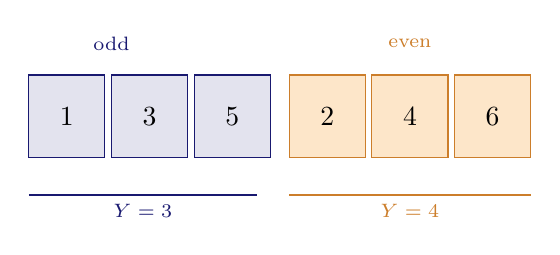
\begin{tikzpicture}[x=1.05cm,y=1.05cm]
  \foreach \i/\n in {0/1,1/3,2/5} {
    \fill[MidnightBlue!12] (\i,0) rectangle ++(0.92,1);
    \draw[MidnightBlue] (\i,0) rectangle ++(0.92,1);
    \node at (\i+0.46,0.5) {$\n$};
  }
  \foreach \i/\n in {3.15/2,4.15/4,5.15/6} {
    \fill[BurntOrange!18] (\i,0) rectangle ++(0.92,1);
    \draw[BurntOrange!80!black] (\i,0) rectangle ++(0.92,1);
    \node at (\i+0.46,0.5) {$\n$};
  }
  \node[font=\scriptsize,MidnightBlue] at (1.0,1.38) {odd};
  \node[font=\scriptsize,BurntOrange!80!black] at (4.61,1.38) {even};
  \draw[MidnightBlue,thick] (0,-0.45) -- (2.76,-0.45);
  \node[font=\scriptsize,below,MidnightBlue] at (1.38,-0.45) {$Y=3$};
  \draw[BurntOrange!80!black,thick] (3.15,-0.45) -- (6.07,-0.45);
  \node[font=\scriptsize,below,BurntOrange!80!black] at (4.61,-0.45) {$Y=4$};
\end{tikzpicture}
